\chapter{NI Vison Assistant}
\label{sec: NI Vison Assistant}


\section{Belichtung}
Als ersten Schritt schauen wir uns an welche Beleuchtung wir verwenden. 
Dafür probieren wir drei verschiedene Beleuchtungen aus.

\subsection{Lampe}
Standard Lampe die im Labor fix montiert ist.
\begin{figure}[H]
    \centering
    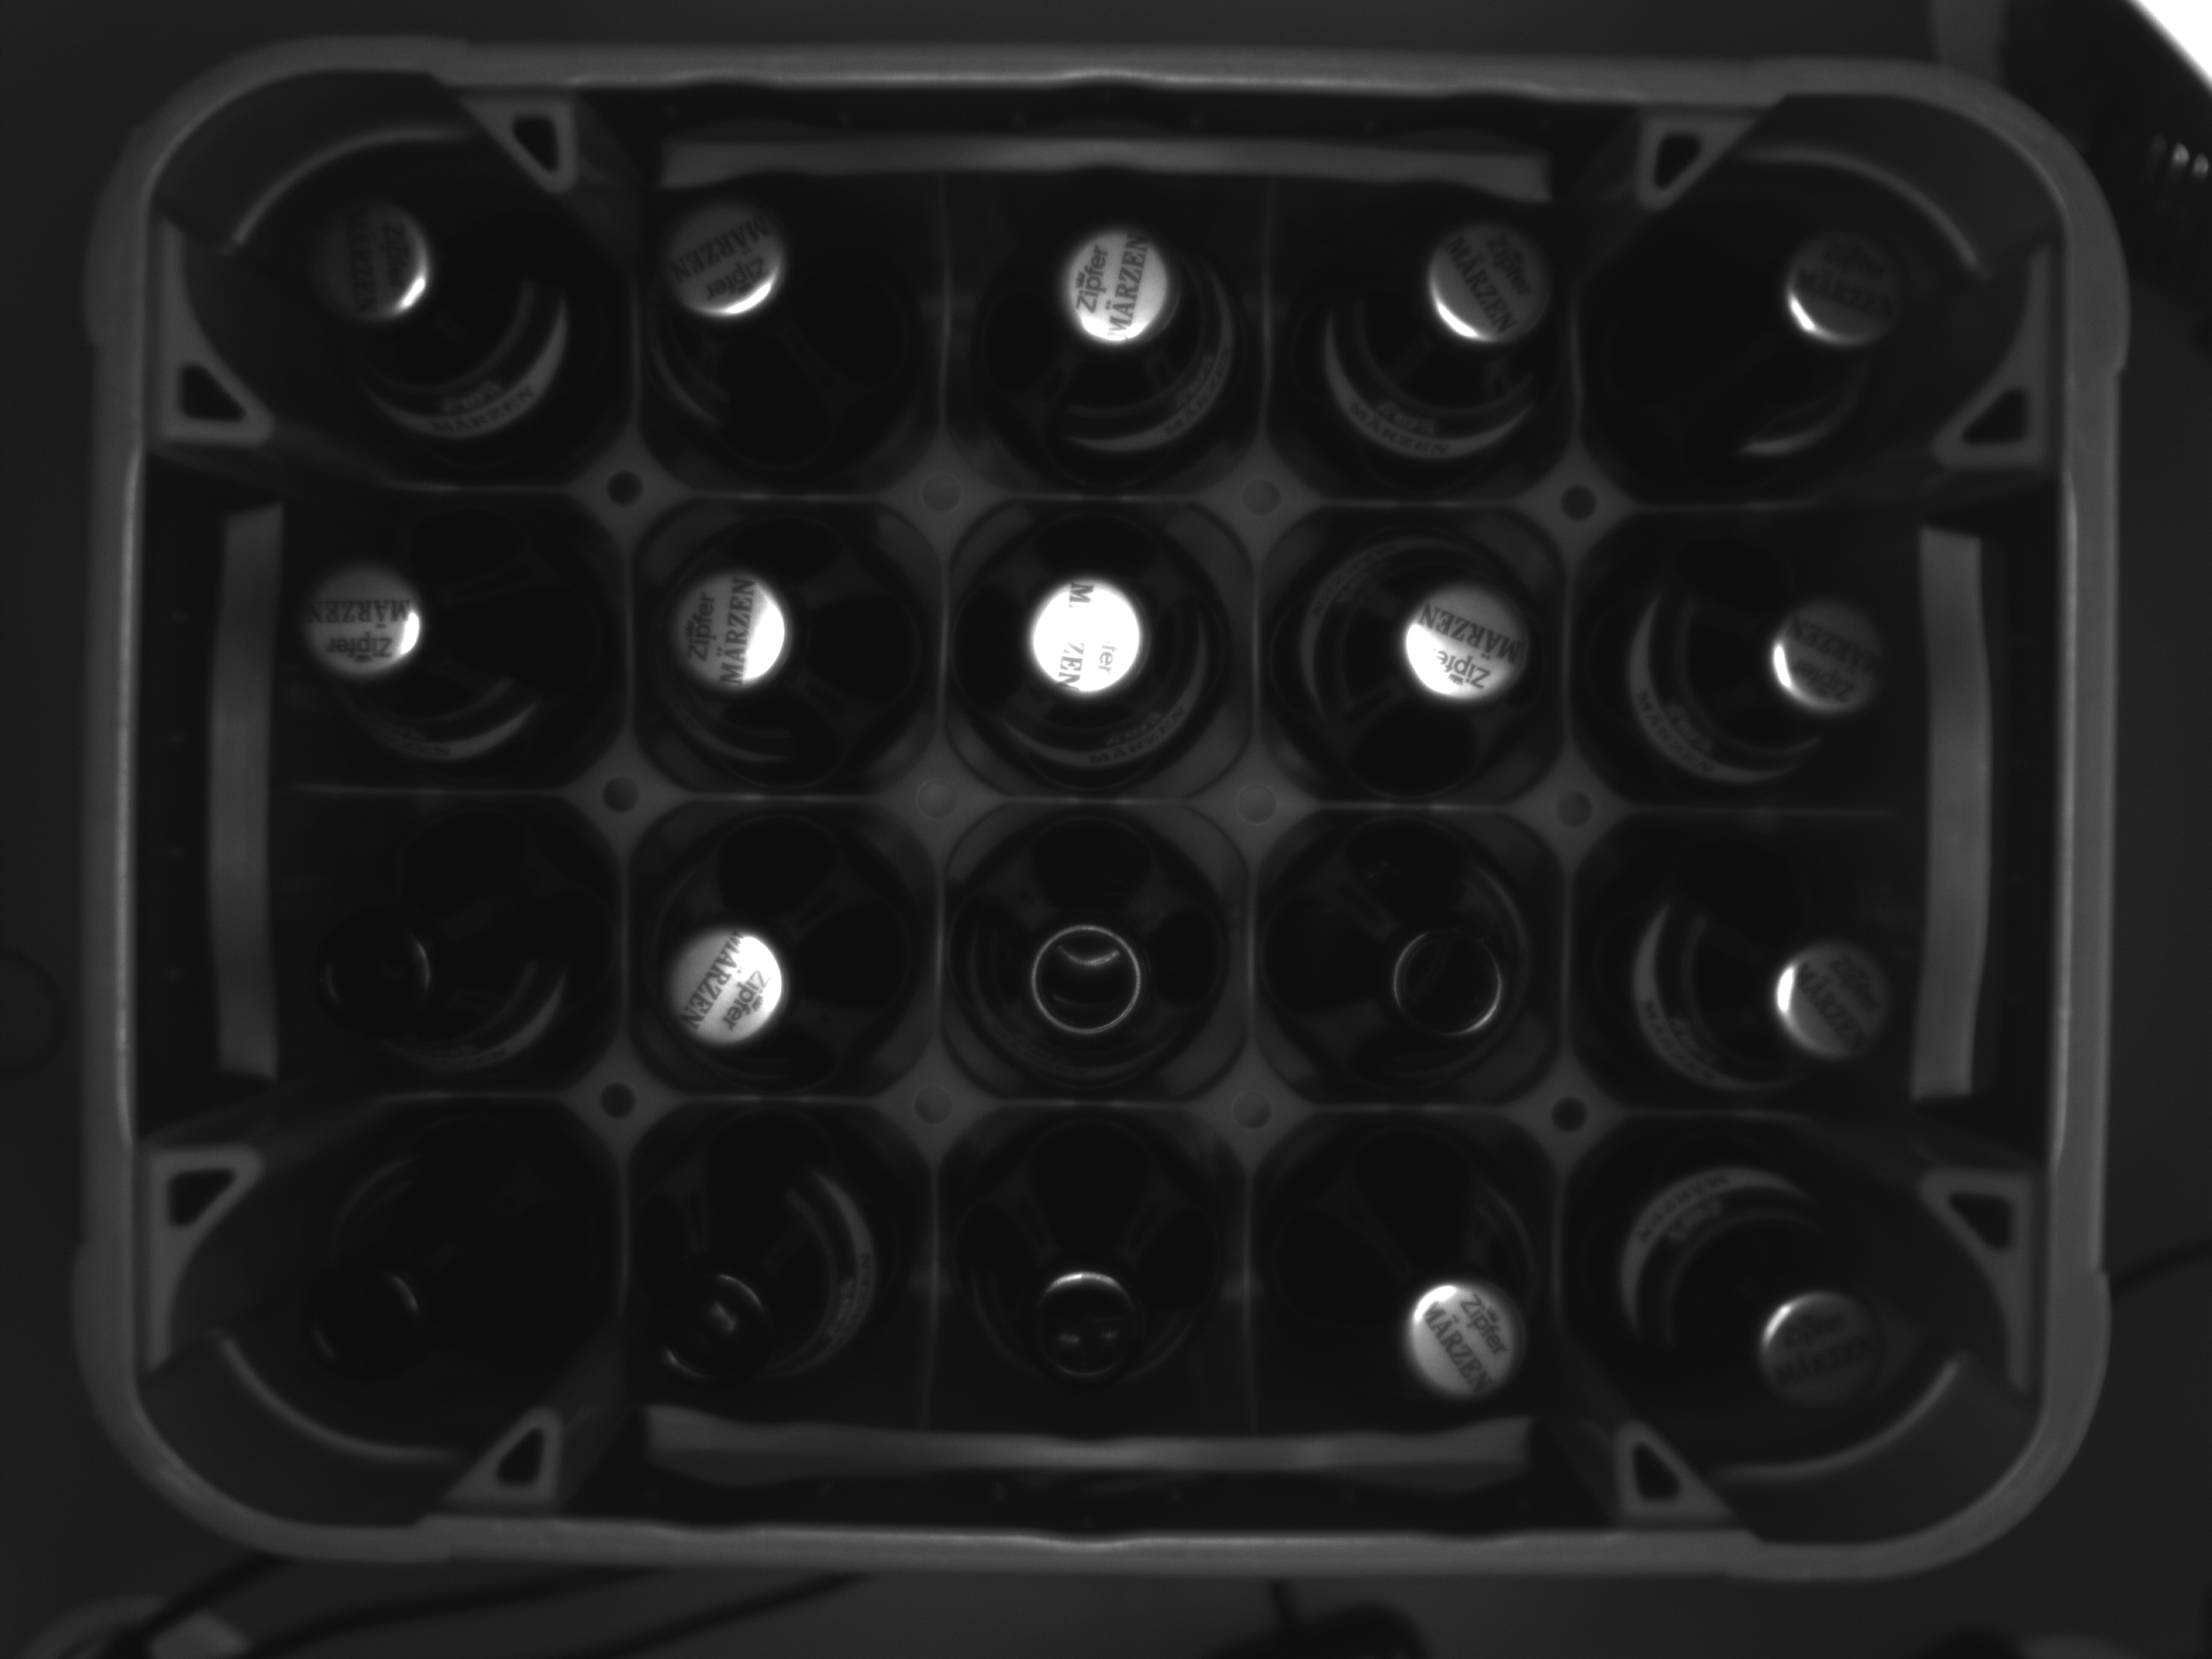
\includegraphics[width=0.6\textwidth]{Grafik/Screenshots_1.Termin_LichtTest&NDI/Lichttest/normales licht.png}
    \caption{Standard Lampe}
    \label{fig:Standard Lampe}
\end{figure}
Man kann hier gut erkennen das nur eine Kapsel wirklich gut reflektiert.

\subsection{Zusätzliche Lampen}
Um mehr Kapseln erkennen zu können leuchten wir händisch mit Taschenlampen zusätzlich.
\begin{figure}[H]
    \centering
    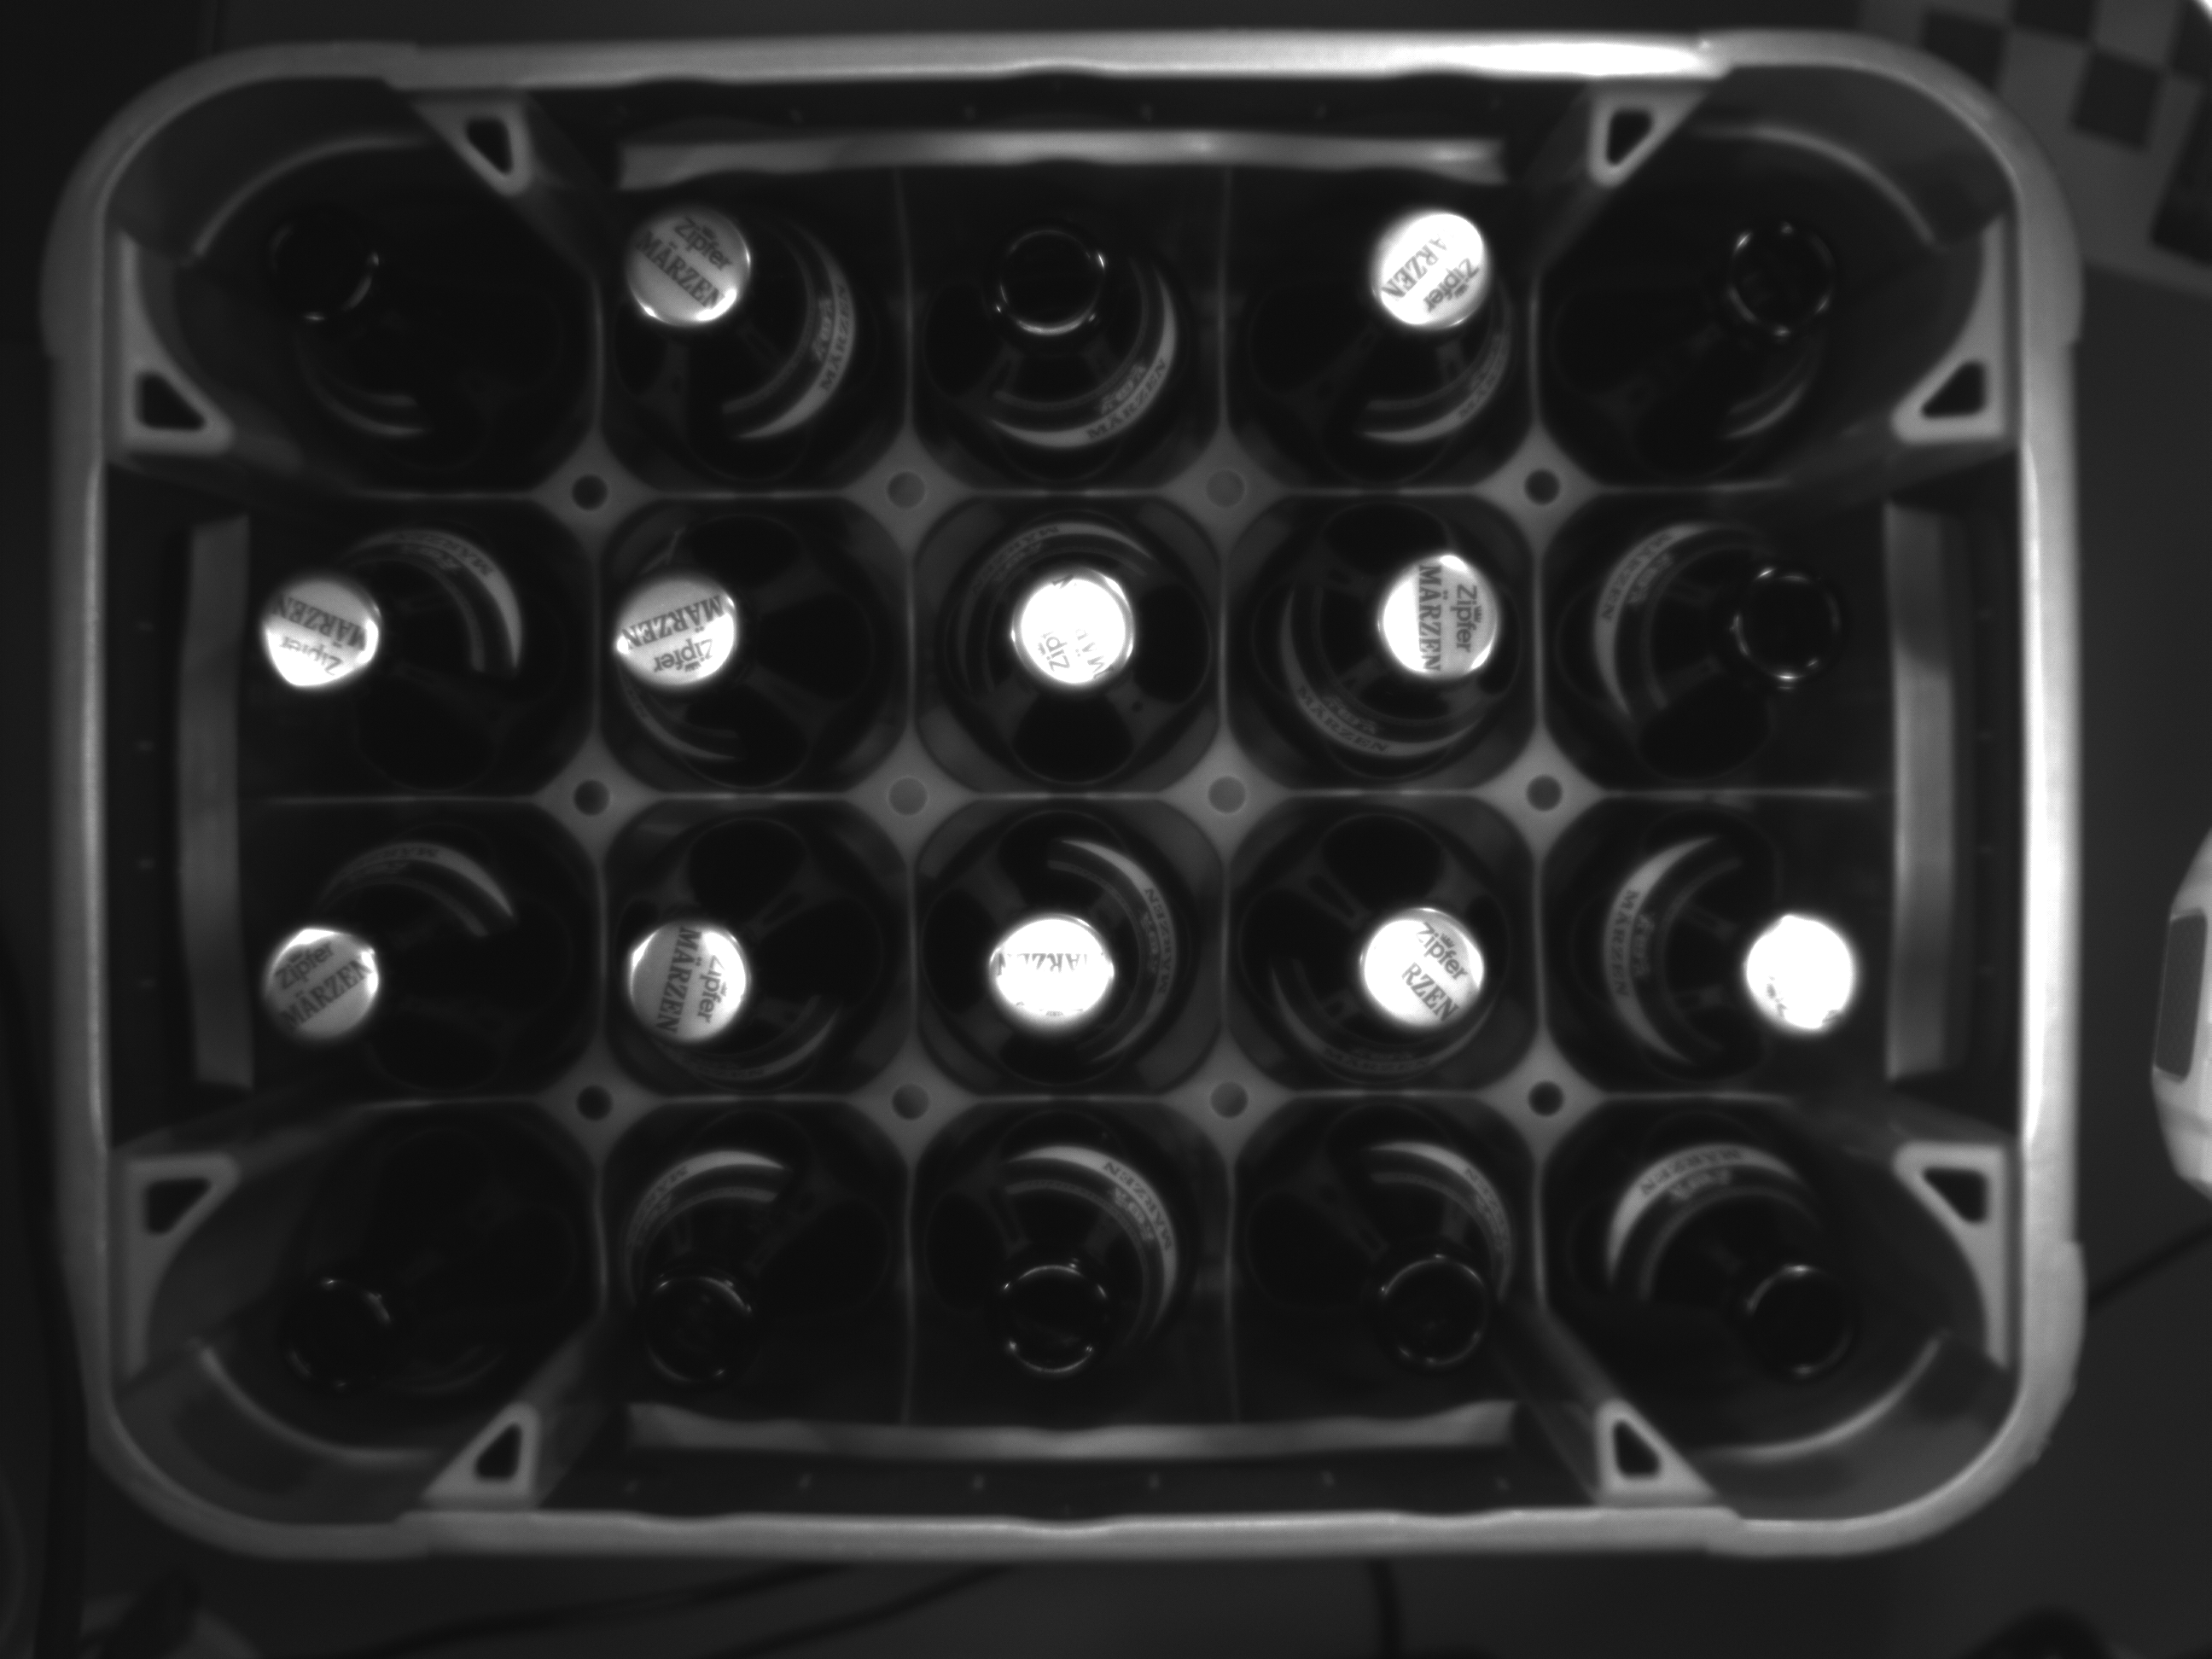
\includegraphics[width=0.6\textwidth]{Grafik/Screenshots_1.Termin_LichtTest&NDI/Lichttest/Mit_Stirnlampen.png}
    \caption{Zusätzliche Lampen}
    \label{fig:Zusätzliche Lampen}
\end{figure}
Mehr Lampen, also mehr Licht, lassen mehr Kapseln reflektieren.

\subsection{Rotlicht}
Eine weitere Idee ist die verwendung einer Rotlichtlampe.
\begin{figure}[H]
    \centering
    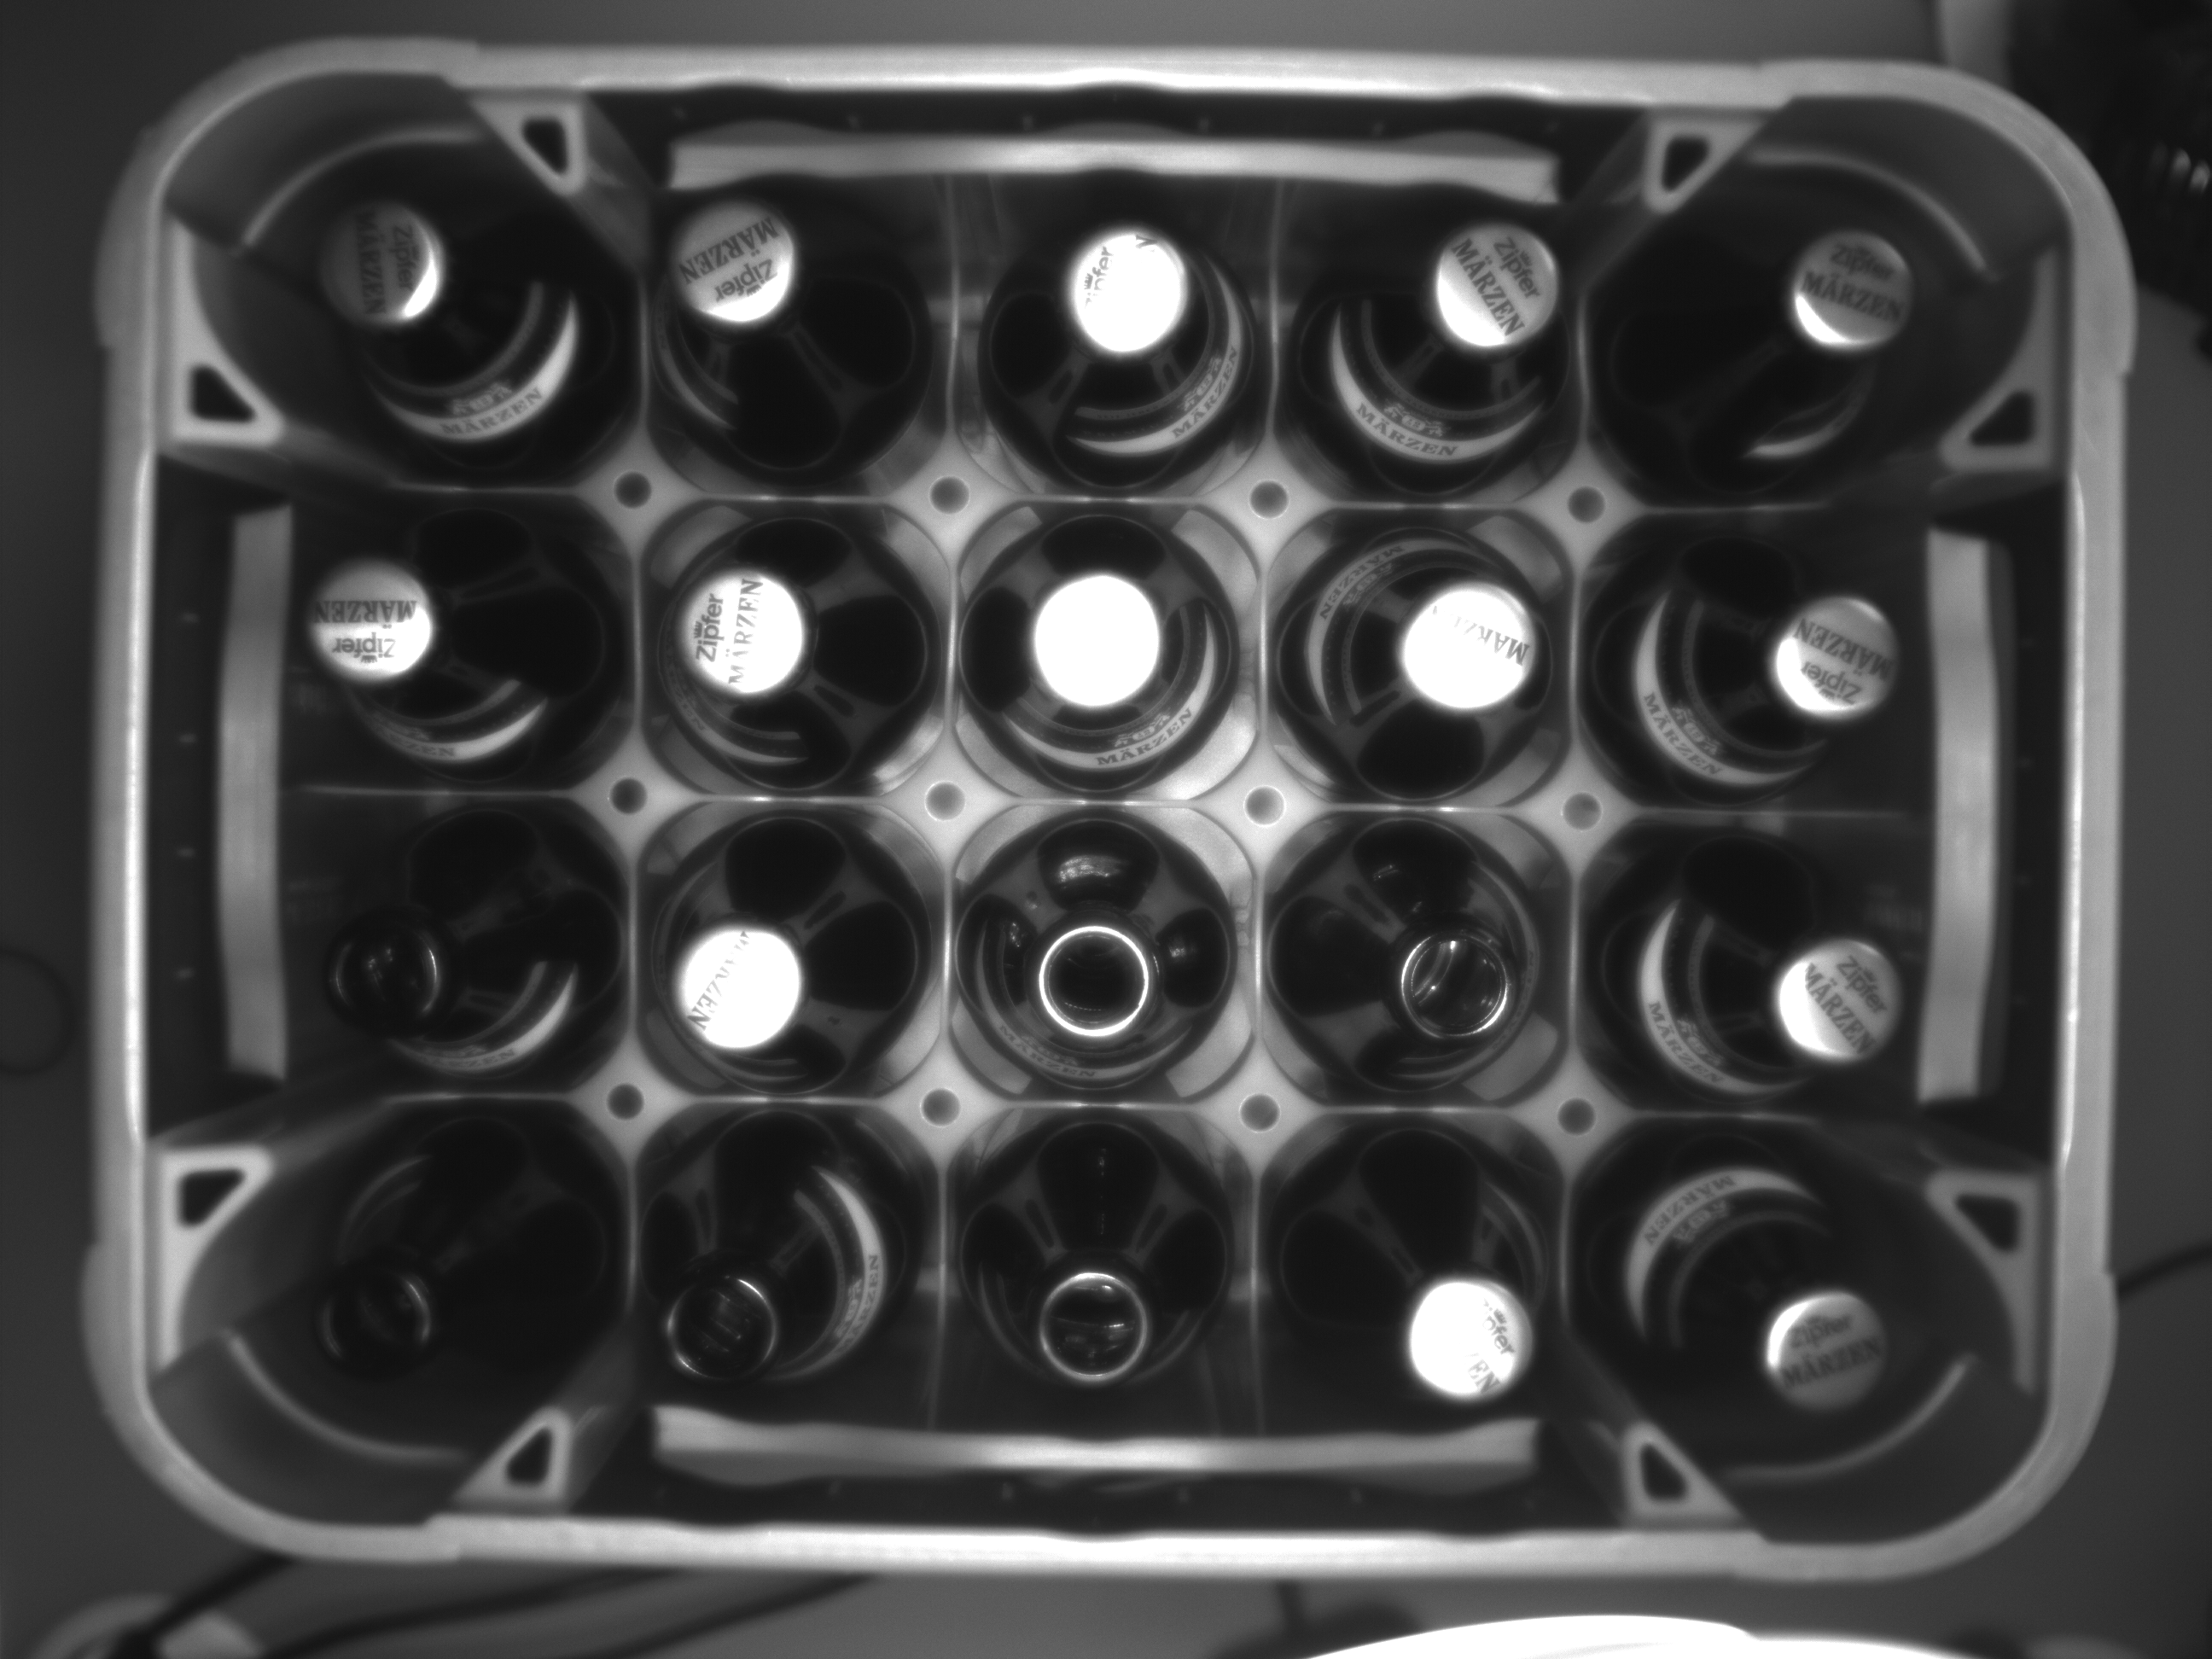
\includegraphics[width=0.6\textwidth]{Grafik/Screenshots_1.Termin_LichtTest&NDI/Lichttest/rotlicht.png}
    \caption{Rotlicht}
    \label{fig:Rotlicht}
\end{figure}
Ähnliches Ergebniss wie vorher.

Wir Entscheiden uns dafür mit der Standard Lampe und zusätzlichen Lampen mit dem VisionAssistant zu starten.


\section{Brightness}
\begin{figure}[H]
    \centering
    \includegraphics[width=0.6\textwidth]{Grafik/Screenshots_2.Termin_NI-VA/1_Brightness.png}
    \caption{}
    \label{fig:}
\end{figure}

\section{Color Plane Extraction}
\begin{figure}[H]
    \centering
    \includegraphics[width=0.6\textwidth]{Grafik/Screenshots_2.Termin_NI-VA/2_ColorPlaneExtraction.png}
    \caption{}
    \label{fig:}
\end{figure}

\section{Threshold}
\begin{figure}[H]
    \centering
    \includegraphics[width=0.6\textwidth]{Grafik/Screenshots_2.Termin_NI-VA/3_Treshold.png}
    \caption{}
    \label{fig:}
\end{figure}



\section{Area Filter}
\begin{figure}[H]
    \centering
    \includegraphics[width=0.6\textwidth]{Grafik/Screenshots_2.Termin_NI-VA/4_AreaFilter.png}
    \caption{}
    \label{fig:}
\end{figure}


\section{Elongation Filter}
\begin{figure}[H]
    \centering
    \includegraphics[width=0.6\textwidth]{Grafik/Screenshots_2.Termin_NI-VA/5_ElongationFilter.png}
    \caption{}
    \label{fig:}
\end{figure}


\section{Convexe Hull}
\begin{figure}[H]
    \centering
    \includegraphics[width=0.6\textwidth]{Grafik/Screenshots_2.Termin_NI-VA/6_ConvexHull.png}
    \caption{}
    \label{fig:}
\end{figure}


\section{Cricle Detection}
\begin{figure}[H]
    \centering
    \includegraphics[width=0.6\textwidth]{Grafik/Screenshots_2.Termin_NI-VA/7_CircleDetection.png}
    \caption{}
    \label{fig:}
\end{figure}